\documentclass[conference,a4paper]{IEEEtran}

\usepackage[T1]{fontenc}
\usepackage{cite}
\usepackage{amsmath,amssymb}
\usepackage{graphicx}
\usepackage{textcomp}
\usepackage{booktabs}
\usepackage{array}
\usepackage{tabularx}
\usepackage{xcolor}
\usepackage{url}
\usepackage{algorithm}
\usepackage{algorithmic}
\usepackage{tikz}
\usetikzlibrary{arrows.meta,positioning,calc,fit,shapes.misc}
\usepackage{balance}
\usepackage{pgfplots}
\pgfplotsset{compat=1.16}


\newcommand{\code}[1]{\texttt{\small #1}}
\newcommand{\sq}{\textquotesingle}
\newcommand{\pii}{p_{99}}

\def\BibTeX{{\rm B\kern-.05em{\sc i\kern-.025em b}\kern-.08em T\kern-.1667em\lower.7ex\hbox{E}\kern-.125emX}}

\begin{document}

\title{Multi-model and NoSQL databases: Evaluating PostgreSQL JSONB, MongoDB, and Redis for Semi-Structured Workloads:  a modern comparison}

\newcommand{\au}[2]{\begin{tabular}[t]{@{}c@{}}
  \normalsize #1\\
  \textit{Dept.\ of Information Technology}\\
  #2
\end{tabular}}

\author{\IEEEauthorblockN{\footnotesize
\begin{tabular}[t]{@{}cc@{}}
\au{Khushpreet Kaur}{Roll No.\ 25124051} \hspace{3em} &
\au{Krish Sharma}{Roll No.\ 25124052} \\
\rule{0pt}{5ex}%
\au{Kamaljeet Singh}{Roll No.\ 25124050} \hspace{3em} &
\au{Jitendra Chaudhary}{Roll No.\ 25124049}
\end{tabular}}}

\maketitle

\begin{abstract}
Many applications pair a relational database for transactions with a document store or an in-memory cache for flexible data and fast reads. PostgreSQL's JSONB type and multi-document transactions in MongoDB have made that split harder to justify. We ran the same synthetic e-commerce order workload on PostgreSQL 16 (JSONB), MongoDB 7.0 and Redis 7.2 at 10,000, 50,000 and 100,000 records, and measured throughput and p50, p95 and p99 latency for batch ingestion, point lookups, filtered scans and field updates. At 100,000 records Redis ingests 161,984 records/s and serves point lookups with a p99 of 0.11\,ms. MongoDB ingests 54,286 records/s, 2.16 times the 25,106 of PostgreSQL, and completes 1,287 field updates/s against 815. We trace that 58\% update gap to MVCC, which writes a whole new tuple for every \code{jsonb\_set} call. On reads PostgreSQL stays within 1.6 times of MongoDB (345 against 557 filtered scans/s) and keeps full relational ACID semantics. At the scales we tested, JSONB removes the need for a separate document store for read-heavy data. Write-heavy services and microsecond-latency tiers still run better on MongoDB and Redis.
\end{abstract}

\begin{IEEEkeywords}
document databases, PostgreSQL JSONB, multi-model databases, NoSQL benchmarking, PACELC, storage engines
\end{IEEEkeywords}

%==========================================================
\section{Introduction}
%==========================================================
Consider the order pipeline of an online retailer. Customer balances must change atomically. Vendor product catalogs arrive in shapes that differ from one merchant to the next. Cart and session state has to come back in under a millisecond. A decade ago the usual answer was polyglot persistence: PostgreSQL for the ledger, MongoDB for catalogs and Redis for sessions. Each tool did did its job, but three clusters brought three problems. A write could succeed in PostgreSQL and fail in MongoDB, leaving the two out of step. The clusters lagged behind each other during synchronization. And a small team had to run backups, upgrades and monitoring for three systems.

Cattell's 2010 survey \cite{cattell2010} describes how this split came about. Relational engines built on normalized schemas and two-phase locking had trouble with horizontal write throughput and with schemas that change weekly. NoSQL stores gave up joins and serializable transactions in return for partitioning, schema freedom and tunable consistency, trade-offs that Brewer's CAP theorem \cite{brewer2012} and Abadi's PACELC \cite{abadi2012} make precise.

The two camps have since moved toward each other. PostgreSQL added JSONB, a parsed binary format for JSON that lives in ordinary table columns and supports indexing. MongoDB added multi-document ACID transactions. This raises a practical question: can a relational engine with JSONB columns replace a dedicated NoSQL engine for semi-structured data, or do its page layout and concurrency control cost too much?

We answer it with three research questions.
\begin{itemize}
\item \textbf{RQ1.} How do CAP and PACELC trade-offs separate key-value, document, wide-column and relational systems in normal operation and during partitions?
\item \textbf{RQ2.} How does PostgreSQL's JSONB storage differ from MongoDB's BSON on WiredTiger, and which storage behaviours set data size, serialization cost and the cost of a partial update?
\item \textbf{RQ3.} When the same semi-structured order workload runs on PostgreSQL JSONB, MongoDB and Redis at 10,000, 50,000 and 100,000 records, how do throughput and the p50, p95 and p99 latencies compare?
\end{itemize}

Our contributions are: (1) a mapping from the consistency theorems to the physical page and memory layouts of each engine; (2) an analysis of how the JSONB format interacts with MVCC; (3) an open benchmark harness that runs identical e-commerce payloads on all three engines; and (4) measurements of throughput and tail latency for batch ingestion, point reads, indexed scans and field updates. Section~II gives the background, Section~III reviews related work, Sections~IV and~V describe the method and the setup, Section~VI reports results and threats to validity, and Section~VII concludes.

%==========================================================
\section{Background}
%==========================================================
\subsection{Data models and distributed consistency}
A relational system stores normalized rows and joins them at query time. A key-value store maps a key to an opaque value with average $O(1)$ access but cannot filter on attributes inside the value. A document store keeps self-describing trees such as JSON or BSON, so nested entities sit inside one record and many joins disappear. A wide-column store keeps sorted column families under a row key, which suits append-heavy data.

CAP \cite{brewer2012} says that during a network partition a replicated store must give up either consistency or availability. Partitions are rare, so PACELC \cite{abadi2012} adds the normal case: if partitioned (P), choose availability (A) or consistency (C); else (E), choose latency (L) or consistency (C). PostgreSQL with synchronous replication is PC/EC, because it pays latency to keep a single order of writes. MongoDB with write concern \code{w:1} acknowledges a write after the primary's memory and journal, before the replicas catch up, so in our configuration it is closest to PC/EL. Published classifications of MongoDB vary with write concern and read preference, so this label applies only to the settings in Section~V. Standalone Redis replicates asynchronously and is PA/EL. Fig.~\ref{fig:pacelc} places the three engines.

\begin{figure}[t]
\centering
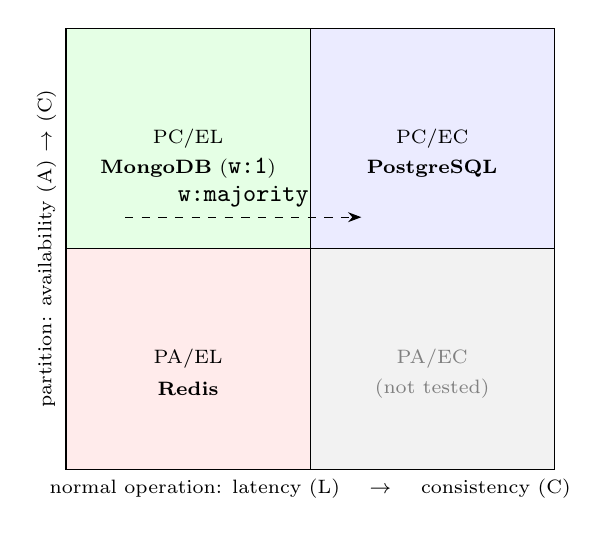
\begin{tikzpicture}[font=\scriptsize,>=Stealth]
\def\w{3.1}\def\h{2.8}
\fill[red!8] (0,0) rectangle (\w,\h);
\fill[green!10] (0,\h) rectangle (\w,2*\h);
\fill[blue!8] (\w,\h) rectangle (2*\w,2*\h);
\fill[gray!10] (\w,0) rectangle (2*\w,\h);
\draw (0,0) rectangle (2*\w,2*\h);
\draw (\w,0)--(\w,2*\h) (0,\h)--(2*\w,\h);
\node at (0.5*\w,0.5*\h) {PA/EL};
\node at (0.5*\w,0.5*\h-0.38) {\textbf{Redis}};
\node at (0.5*\w,1.5*\h) {PC/EL};
\node at (0.5*\w,1.5*\h-0.38) {\textbf{MongoDB} (\code{w:1})};
\node at (1.5*\w,1.5*\h) {PC/EC};
\node at (1.5*\w,1.5*\h-0.38) {\textbf{PostgreSQL}};
\node[gray] at (1.5*\w,0.5*\h) {PA/EC};
\node[gray] at (1.5*\w,0.5*\h-0.38) {(not tested)};
\draw[->,dashed] (0.5*\w-0.8,1.5*\h-1.0) -- (1.5*\w-0.9,1.5*\h-1.0) node[midway,above,font=\tiny] {\code{w:majority}};
\node[below] at (\w,0) {normal operation: latency (L) \quad $\rightarrow$ \quad consistency (C)};
\node[rotate=90,above] at (0,\h) {partition: availability (A) $\rightarrow$ (C)};
\end{tikzpicture}
\caption{PACELC placement of the three engines in the configurations we tested.}
\label{fig:pacelc}
\end{figure}

\subsection{Storage engines and JSONB internals}
B-trees and B+ trees organize data into pages that match the disk block, 8\,KB in PostgreSQL and 4 to 32\,KB in WiredTiger. They give $O(\log N)$ lookups but cause write amplification from random page updates and log flushes. Log-structured merge trees, used by RocksDB and Cassandra, buffer writes in a memtable and flush sorted immutable files, which favours ingestion at the price of multi-level reads and background compaction. We did not test an LSM engine. Redis keeps all keys in an in-memory hash table with incremental rehashing and uses skip lists for sorted sets.

PostgreSQL's plain \code{json} type stores the exact text and re-parses it on every access. JSONB, introduced in version 9.4, stores a parsed tree: a 32-bit header holding the element count and container type, an array of 32-bit JEntry descriptors with types and offsets, and the payload bytes (Fig.~\ref{fig:layouts}b). Object keys are sorted at write time, so the executor can binary-search them in $O(\log K)$ without parsing earlier entries. A GIN index with \code{jsonb\_ops} indexes every key and value. The \code{jsonb\_path\_ops} variant hashes root-to-leaf paths instead and builds a smaller index for containment queries.

Rows live in fixed 8\,KB slotted pages with a 24-byte header and 4-byte line pointers that point to tuples packed from the end of the page (Fig.~\ref{fig:layouts}a). Under MVCC a tuple is never edited in place. A \code{jsonb\_set()} call builds a new heap tuple that contains the whole document and leaves the old tuple for \code{VACUUM}. Because our workload updates an indexed expression (\code{status}), the heap-only-tuple shortcut does not apply and new index entries are written as well.

WiredTiger keeps B-tree pages in an in-memory cache, and worker threads pin the pages they use with hazard pointers so that eviction threads leave them alone. A field update adds a small modify record to the key's in-memory update chain and writes an operation-level record to the journal. The page itself is rewritten only at a checkpoint, by default every 60 seconds (Fig.~\ref{fig:layouts}c). In Redis each record is a \code{dictEntry} that points to a 16-byte \code{robj} and a simple dynamic string allocated by jemalloc (Fig.~\ref{fig:layouts}d). Nothing is translated to disk pages, but rewriting a variable-length string forces a reallocation and fragments the jemalloc arenas over time.

\begin{figure*}[t]
\centering
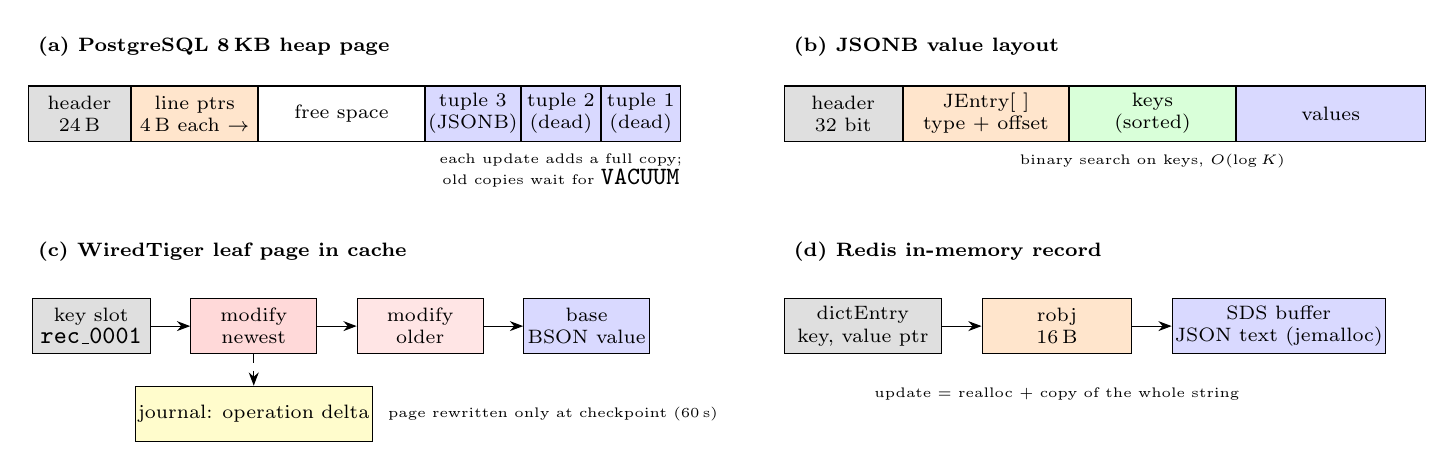
\begin{tikzpicture}[font=\scriptsize,>=Stealth,
  blk/.style={draw,minimum height=7mm,align=center,inner sep=1pt},
  ttl/.style={font=\scriptsize\bfseries,anchor=west}]
% (a) PostgreSQL page
\node[ttl] at (0,1.25) {(a) PostgreSQL 8\,KB heap page};
\node[blk,fill=gray!25,minimum width=1.3cm] (a1) at (0.65,0.4) {header\\24\,B};
\node[blk,fill=orange!20,minimum width=1.6cm,right=0pt of a1] (a2) {line ptrs\\4\,B each $\rightarrow$};
\node[blk,fill=white,minimum width=2.1cm,right=0pt of a2] (a3) {free space};
\node[blk,fill=blue!15,minimum width=1.0cm,right=0pt of a3] (a4) {tuple 3\\(JSONB)};
\node[blk,fill=blue!15,minimum width=1.0cm,right=0pt of a4] (a5) {tuple 2\\(dead)};
\node[blk,fill=blue!15,minimum width=1.0cm,right=0pt of a5] (a6) {tuple 1\\(dead)};
\node[font=\tiny,below=1pt of a5,text width=5cm,align=center] {each update adds a full copy; old copies wait for \code{VACUUM}};
% (b) JSONB value
\node[ttl] at (9.6,1.25) {(b) JSONB value layout};
\node[blk,fill=gray!25,minimum width=1.5cm] (b1) at (10.35,0.4) {header\\32 bit};
\node[blk,fill=orange!20,minimum width=2.1cm,right=0pt of b1] (b2) {JEntry[ ]\\type + offset};
\node[blk,fill=green!15,minimum width=2.1cm,right=0pt of b2] (b3) {keys\\(sorted)};
\node[blk,fill=blue!15,minimum width=2.4cm,right=0pt of b3] (b4) {values};
\node[font=\tiny,below=1pt of b3,text width=5cm,align=center] {binary search on keys, $O(\log K)$};
% (c) WiredTiger
\node[ttl] at (0,-1.35) {(c) WiredTiger leaf page in cache};
\node[blk,fill=gray!25,minimum width=1.5cm] (c1) at (0.8,-2.3) {key slot\\\code{rec\_0001}};
\node[blk,fill=red!15,minimum width=1.6cm,right=0.5cm of c1] (c2) {modify\\newest};
\node[blk,fill=red!10,minimum width=1.6cm,right=0.5cm of c2] (c3) {modify\\older};
\node[blk,fill=blue!15,minimum width=1.6cm,right=0.5cm of c3] (c4) {base\\BSON value};
\draw[->] (c1)--(c2); \draw[->] (c2)--(c3); \draw[->] (c3)--(c4);
\node[blk,fill=yellow!20,minimum width=2.6cm,below=4mm of c2] (c5) {journal: operation delta};
\draw[->,dashed] (c2)--(c5);
\node[font=\tiny,right=2pt of c5,text width=4.2cm] {page rewritten only at checkpoint (60\,s)};
% (d) Redis
\node[ttl] at (9.6,-1.35) {(d) Redis in-memory record};
\node[blk,fill=gray!25,minimum width=2.0cm] (d1) at (10.6,-2.3) {dictEntry\\key, value ptr};
\node[blk,fill=orange!20,minimum width=1.9cm,right=0.5cm of d1] (d2) {robj\\16\,B};
\node[blk,fill=blue!15,minimum width=2.6cm,right=0.5cm of d2] (d3) {SDS buffer\\JSON text (jemalloc)};
\draw[->] (d1)--(d2); \draw[->] (d2)--(d3);
\node[font=\tiny,below=3mm of d2,text width=6cm,align=center] {update = realloc + copy of the whole string};
\end{tikzpicture}
\caption{Physical layouts of the three engines. (a) and (b) show how PostgreSQL stores a JSONB document. (c) and (d) show the update paths in WiredTiger and Redis.}
\label{fig:layouts}
\end{figure*}

%==========================================================
\section{Related Work}
%==========================================================
We reviewed 17 peer-reviewed studies published between 2010 and 2026 in venues such as ACM SIGMOD, VLDB, IEEE TKDE and IEEE ICDE; 11 of them appeared in 2021 or later. They fall into three themes.

\subsection{Consistency and latency in distributed stores}
Research on distributed stores starts from Cattell's survey \cite{cattell2010} and from CAP and PACELC \cite{brewer2012,abadi2012}. Cooper et al.\ introduced YCSB \cite{cooper2010} and showed that key-value and document stores reach high throughput by relaxing ACID guarantees. Silva et al.\ \cite{silva2025} measured PACELC latency distributions under cloud network jitter and found that synchronous replication raises $p_{99}$ while replicas synchronize. Kumar and Gokhale \cite{kumar2023} benchmarked NoSQL and NewSQL engines: NewSQL restored serializable transactions but trailed document stores in write throughput by 2.4 to 3.8 times because of consensus coordination.

\subsection{Multi-model architectures}
Multi-model systems try to hold several data models in one engine. Ong et al.\ proposed SQL++ \cite{ong2014}, a single language for flat tables and nested JSON. Lu and Holubov\'a \cite{lu2019} split such systems into extended relational engines, PostgreSQL JSONB among them, and native multi-model engines like ArangoDB. Wang et al.\ \cite{wang2021} built UniBench and found that cross-model queries in extended relational systems pay for translating between tables and nested objects. Liu et al.\ \cite{liu2022} report that serializable transactions over mixed document and relational records cost about 35\% of throughput. Martinez and Fernandez \cite{martinez2026} survey how relational systems gained document types while NoSQL engines gained transactions.

\subsection{Semi-structured storage and indexing}
Zhang et al.\ \cite{zhang2021} built path-filtering index trees that cut GIN storage by 45\% at the same selectivity. Ren et al.\ \cite{ren2022} applied columnar dictionary compression to JSON attributes and reached a 2.8 times compression ratio, with 22\% lower write throughput. Al-Sayed et al.\ \cite{alsayed2023} compared MongoDB, Couchbase and PostgreSQL JSONB. PostgreSQL matched the document stores on point reads and trailed on writes. Chen et al.\ \cite{chen2024} traced that to immutable MVCC row versions, which force full tuple copies, and showed that partial delta logging improves updates by 3.2 times in a prototype that is not in mainline PostgreSQL. Wu et al.\ \cite{wu2024} compared B-trees and LSM-trees on NVMe: LSM-trees wrote 4 times faster and B-trees read points with 60\% lower latency. Zhao et al.\ \cite{zhao2025} sped up in-memory JSON parsing 8 times with SIMD instructions.

\begin{table*}[t]
\caption{Comparison of ten key related studies}
\label{tab:lit}
\centering
\footnotesize
\begin{tabularx}{\textwidth}{@{}p{2.5cm}p{2.9cm}p{4.4cm}X@{}}
\toprule
Study & Subject & Key finding & Gap \\
\midrule
Abadi 2012 \cite{abadi2012} & PACELC formulation & Latency versus consistency trade-off persists without partitions & Theory only, no micro-benchmarks \\
Cooper et al.\ 2010 \cite{cooper2010} & YCSB on Cassandra, HBase, PNUTS, MySQL & Six standard cloud workloads & Flat key-value records, no nested documents \\
Wang et al.\ 2021 \cite{wang2021} & UniBench on PostgreSQL, ArangoDB & Cross-model joins slow relational JSON by 2.1 times & Graph and document hybrid, no in-memory store \\
Zhang et al.\ 2021 \cite{zhang2021} & Adaptive JSON path indexing & GIN footprint reduced by 45\% & Read queries only, no in-place updates \\
Liu et al.\ 2022 \cite{liu2022} & Multi-model transaction isolation & Serializable mode costs 35\% throughput & Synthetic workloads, no Redis \\
Ren et al.\ 2022 \cite{ren2022} & Columnar dictionary encoding for JSON & 2.8 times compression, 22\% slower writes & Read-focused evaluation \\
Al-Sayed et al.\ 2023 \cite{alsayed2023} & MongoDB, Couchbase, PostgreSQL & PostgreSQL competitive on point lookups, behind on writes & No sub-millisecond caching tier \\
Chen et al.\ 2024 \cite{chen2024} & Delta WAL for binary JSON & 3.2 times faster updates & Prototype, not in mainline PostgreSQL \\
Wu et al.\ 2024 \cite{wu2024} & B-tree versus LSM on NVMe & LSM 4 times faster writes, B-tree 60\% lower read latency & Storage tier only \\
Zhao et al.\ 2025 \cite{zhao2025} & SIMD JSON parsing & 8 times faster queries with AVX-512 & Pure in-memory, no durability \\
\bottomrule
\end{tabularx}
\end{table*}

\subsection{Research gap}
Earlier work evaluated multi-model query languages \cite{ong2014}, surveyed taxonomies \cite{lu2019,martinez2026} or benchmarked flat key-value records \cite{cooper2010}. Table~\ref{tab:lit} shows what is still missing. No study we found runs identical semi-structured e-commerce workloads on PostgreSQL 16 (JSONB), MongoDB 7.0 and Redis 7.2 on controlled hardware and reports $p_{99}$ for batch insertion, point lookup, filtered scan and in-place update together. Most earlier benchmarks used older engine versions, flat records or mean latency alone.

%==========================================================
\section{Methodology}
%==========================================================
\subsection{System architecture}
Fig.~\ref{fig:arch} shows the harness. A seeded generator produces the same order documents for every run. A thin adapter per engine sends them to PostgreSQL, MongoDB or Redis, each in its own container on the same host, and a timer records every operation.

\begin{figure}[t]
\centering
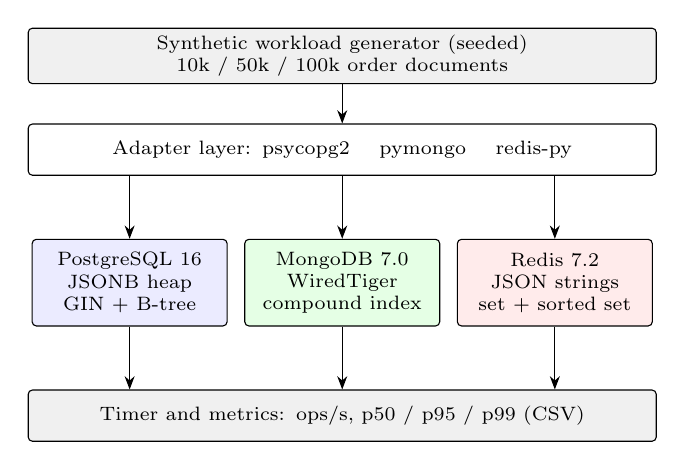
\begin{tikzpicture}[font=\scriptsize,>=Stealth,
  box/.style={draw,rounded corners=1.5pt,align=center,inner sep=2.5pt,minimum height=6.5mm},
  eng/.style={box,text width=2.3cm,minimum height=11mm}]
\node[box,fill=gray!12,text width=7.8cm] (gen) {Synthetic workload generator (seeded)\\10k / 50k / 100k order documents};
\node[box,below=5mm of gen,text width=7.8cm] (drv) {Adapter layer: psycopg2 \quad pymongo \quad redis-py};
\node[eng,fill=blue!8,below=8mm of drv,xshift=-2.7cm] (pg) {PostgreSQL 16\\JSONB heap\\GIN + B-tree};
\node[eng,fill=green!10,below=8mm of drv] (mg) {MongoDB 7.0\\WiredTiger\\compound index};
\node[eng,fill=red!8,below=8mm of drv,xshift=2.7cm] (rd) {Redis 7.2\\JSON strings\\set + sorted set};
\node[box,fill=gray!12,below=8mm of mg,text width=7.8cm] (met) {Timer and metrics: ops/s, p50 / p95 / p99 (CSV)};
\draw[->] (gen)--(drv);
\foreach \n in {pg,mg,rd}{
  \draw[->] (\n.north |- drv.south)--(\n.north);
  \draw[->] (\n.south)--(\n.south |- met.north);}
\end{tikzpicture}
\caption{Architecture of the benchmark harness.}
\label{fig:arch}
\end{figure}

\subsection{Workload and schema mapping}
Each record is a retail order with a customer ID, timestamp, status, total, a list of one to four line items and client metadata:

\noindent\begin{minipage}{\columnwidth}\footnotesize
\begin{verbatim}
{ "id": "rec_00045210", "customer_id": "cust_82419",
  "created_at": "2026-11-10T05:28:30Z",
  "status": "shipped", "total_amount": 348.50,
  "items": [{"sku": "SKU-4912", "category":
     "electronics", "qty": 2, "unit_price": 149.25}, ...],
  "metadata": {"device": "mobile_ios", "session_id":
     "a9f82d1c", "loyalty_tier": "platinum",
     "fraud_score": 0.042} }
\end{verbatim}\end{minipage}\par\vspace{3pt}

PostgreSQL stores the document in \code{orders\_jsonb(id VARCHAR(64) PRIMARY KEY, data JSONB NOT NULL)} with a GIN index using \code{jsonb\_path\_ops} and an expression B-tree on \code{(data->>\sq status\sq)} and \code{((data->>\sq total\_amount\sq)::numeric)}. MongoDB stores it in the \code{orders} collection with \code{\_id} set to the order ID and a compound index on \code{\{status:1, total\_amount:1\}}. Redis stores a JSON string under \code{order:\{id\}}, keeps a set \code{idx:status:\{status\}} of matching IDs and a sorted set \code{idx:amount} scored by \code{total\_amount}.

\subsection{Queries}
Table~\ref{tab:queries} lists the three query types that ran on every engine.

\begin{table*}[t]
\caption{Query syntax used on each engine}
\label{tab:queries}
\centering
\scriptsize
\newcommand{\cl}[1]{\begin{tabular}[t]{@{}l@{}}#1\end{tabular}}
\newcommand{\tc}[1]{\texttt{#1}}
\renewcommand{\arraystretch}{1.2}
\begin{tabular}{@{}p{1.7cm}p{6.0cm}p{4.9cm}p{4.2cm}@{}}
\toprule
Operation & PostgreSQL & MongoDB & Redis \\
\midrule
Point lookup &
\cl{\tc{SELECT data FROM orders\_jsonb}\\\tc{WHERE id = \sq rec\_00010000\sq;}} &
\cl{\tc{db.orders.find(}\\\tc{\{\_id: \sq rec\_00010000\sq\})}} &
\tc{GET order:rec\_00010000} \\
Filtered scan &
\cl{\tc{SELECT data FROM orders\_jsonb}\\\tc{WHERE data->>\sq status\sq = \sq shipped\sq}\\\tc{AND (data->>\sq total\_amount\sq)::numeric}\\\tc{\ \ >= 100.0 LIMIT 50;}} &
\cl{\tc{db.orders.find(\{status:\sq shipped\sq,}\\\tc{\ \ total\_amount:\{\$gte:100.0\}\})}\\\tc{.limit(50)}} &
\cl{\tc{ZRANGEBYSCORE idx:amount}\\\tc{100.0 +inf LIMIT 0 50}} \\
Field update &
\cl{\tc{UPDATE orders\_jsonb SET data =}\\\tc{jsonb\_set(data, \sq\{status\}\sq,}\\\tc{\sq\char34{} cancelled\char34{}\sq)}\\\tc{WHERE id = \sq rec\_00010000\sq;}} &
\cl{\tc{db.orders.updateOne(}\\\tc{\{\_id:\sq rec\_00010000\sq\},}\\\tc{\{\$set:\{status:\sq cancelled\sq\}\})}} &
\cl{\tc{GET order:rec\_00010000;}\\change JSON in the client;\\\tc{SET order:rec\_00010000}} \\
\bottomrule
\end{tabular}
\end{table*}

\subsection{Execution procedure}
Algorithm~\ref{alg:bench} gives the procedure. Records go in batches of 1,000, which balances packet utilization against engine buffer use. Indexes are built after ingestion. The scan loop draws a random status and a random minimum total between 50 and 200, and the update loop rewrites the status of 250 sampled records. All clients are native drivers (\code{psycopg2-binary}, \code{pymongo}, \code{redis-py}). We avoided ORMs because their object mapping adds overhead that hides engine behaviour.

\begin{algorithm}[t]
\caption{Ingestion, scan and update pipeline}
\label{alg:bench}
\begin{algorithmic}[1]
\REQUIRE size $N\in\{10\text{k},50\text{k},100\text{k}\}$, batch $B=1000$, scans $M=50$, updates $U=250$
\STATE $D \leftarrow \textsc{GenerateRecords}(N)$
\FOR{each chunk $C$ of $B$ records in $D$}
  \STATE $t_0 \leftarrow$ timer;\; \textsc{BatchInsert}$(C)$;\; record $\Delta t$
\ENDFOR
\STATE \textsc{BuildSecondaryIndexes}()
\FOR{$i = 1$ \TO $M$}
  \STATE $s \leftarrow$ random status;\; $a \leftarrow$ uniform$(50,200)$
  \STATE time \textsc{Scan}$(\text{status}=s,\ \text{total}\ge a,\ \text{limit }50)$
\ENDFOR
\FOR{each record $r$ in a sample of $U$}
  \STATE time \textsc{Update}$(r,\ \text{status}\leftarrow\text{cancelled})$
\ENDFOR
\STATE compute throughput and $p_{50},p_{95},p_{99}$ (interpolated)
\end{algorithmic}
\end{algorithm}

%==========================================================
\section{Experimental Setup}
%==========================================================
All runs used one dedicated machine with four physical cores at 3.60\,GHz, 16\,GB of DDR4-3200 memory, a 512\,GB PCIe 4.0 NVMe drive (3,500\,MB/s sequential read, 3,000\,MB/s sequential write) and 64-bit Linux 5.15, with each database in a container. Table~\ref{tab:config} gives the engine settings.

\begin{table}[t]
\caption{Engine versions and configuration}
\label{tab:config}
\centering
\footnotesize
\begin{tabularx}{\columnwidth}{@{}l>{\raggedright\arraybackslash}X@{}}
\toprule
Engine & Settings \\
\midrule
PostgreSQL 16 & \code{shared\_buffers=512MB}, \code{work\_mem=64MB}, \code{maintenance\_work\_mem=128MB}, \code{synchronous\_commit=off} \\
MongoDB 7.0 & WiredTiger cache 1.0\,GB, journal on, read concern \code{local}, write concern \code{w:1} \\
Redis 7.2 & \code{maxmemory=1GB}, \code{allkeys-lru}, snapshots disabled \\
\bottomrule
\end{tabularx}
\end{table}

We turned off synchronous commit in PostgreSQL and snapshots in Redis so that the results reflect memory and page handling instead of disk stalls. The dataset is synthetic, so no personal data is involved. At 10,000, 50,000 and 100,000 records it occupies 4.8, 24.1 and 48.2\,MB of raw JSON, about 0.48\,KB per record, and fits in every engine's cache. For each operation we record throughput in operations per second and the p50, p95 and p99 latency with continuous percentile interpolation. Batch-insert latencies are per batch of 1,000 records.

%==========================================================
\section{Results and Discussion}
%==========================================================
Table~\ref{tab:results} reports the 100,000-record results, Fig.~\ref{fig:bars} plots them, Table~\ref{tab:scale} and Fig.~\ref{fig:scale} show how they change with scale, and Fig.~\ref{fig:update} compares the update paths.

\begin{table}[t]
\caption{Results at 100,000 records}
\label{tab:results}
\centering
\footnotesize
\setlength{\tabcolsep}{3.5pt}
\begin{tabular}{@{}llrrrr@{}}
\toprule
Engine & Operation & ops/s & vs.\ PG & $p_{50}$ (ms) & $p_{99}$ (ms) \\
\midrule
PostgreSQL & Batch insert & 25,105.8 & 1.00 & 39.71 & 56.54 \\
(JSONB)    & Point lookup & 1,520.0 & 1.00 & 0.65 & 1.02 \\
           & Filtered scan & 345.1 & 1.00 & 2.94 & 3.72 \\
           & Field update & 814.7 & 1.00 & 1.24 & 1.76 \\
\midrule
MongoDB    & Batch insert & 54,286.1 & 2.16 & 18.25 & 25.67 \\
(WiredTiger) & Point lookup & 2,184.2 & 1.44 & 0.45 & 0.68 \\
           & Filtered scan & 557.3 & 1.61 & 1.79 & 2.30 \\
           & Field update & 1,287.3 & 1.58 & 0.77 & 1.18 \\
\midrule
Redis      & Batch insert & 161,984.4 & 6.45 & 6.16 & 8.01 \\
(in-memory) & Point lookup & 12,398.4 & 8.16 & 0.08 & 0.11 \\
           & Filtered scan & 1,316.7 & 3.82 & 0.76 & 0.95 \\
           & Field update & 6,895.5 & 8.46 & 0.14 & 0.23 \\
\bottomrule
\end{tabular}
\end{table}

\begin{figure*}[t]
\centering
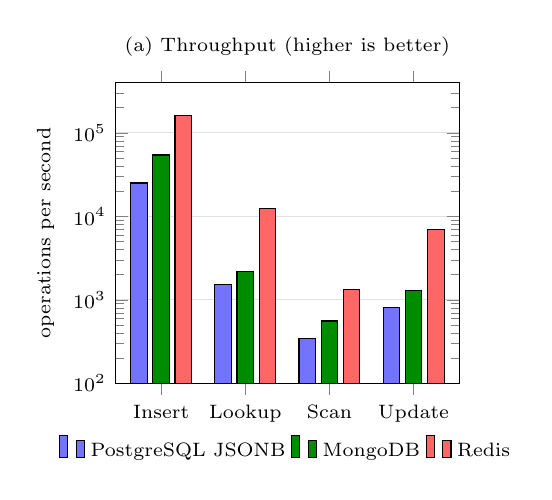
\begin{tikzpicture}
\begin{axis}[ybar,log origin=infty,width=0.49\textwidth,height=5.4cm,ymode=log,ymin=100,ymax=400000,
  bar width=6pt,symbolic x coords={Insert,Lookup,Scan,Update},xtick=data,enlarge x limits=0.18,
  ylabel={operations per second},title={(a) Throughput (higher is better)},
  tick label style={font=\scriptsize},label style={font=\scriptsize},title style={font=\scriptsize},
  legend style={font=\scriptsize,at={(0.5,-0.15)},anchor=north,legend columns=-1,draw=none},
  ymajorgrids,grid style={gray!25}]
\addplot[fill=blue!55,draw=black] coordinates {(Insert,25105.8)(Lookup,1520.0)(Scan,345.1)(Update,814.7)};
\addplot[fill=green!55!black,draw=black] coordinates {(Insert,54286.1)(Lookup,2184.2)(Scan,557.3)(Update,1287.3)};
\addplot[fill=red!60,draw=black] coordinates {(Insert,161984.4)(Lookup,12398.4)(Scan,1316.7)(Update,6895.5)};
\legend{PostgreSQL JSONB,MongoDB,Redis}
\end{axis}
\end{tikzpicture}\hfill
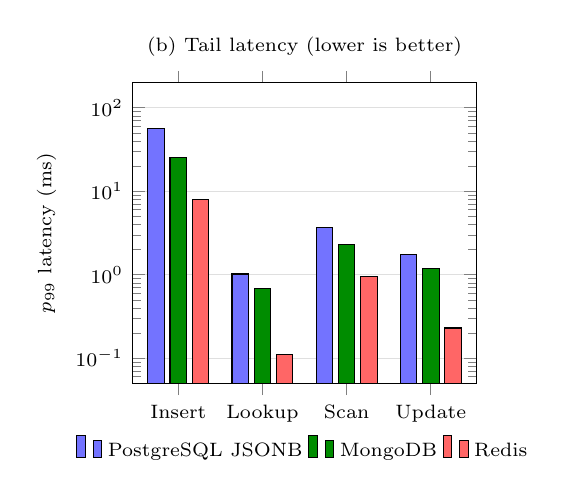
\begin{tikzpicture}
\begin{axis}[ybar,log origin=infty,width=0.49\textwidth,height=5.4cm,ymode=log,ymin=0.05,ymax=200,
  bar width=6pt,symbolic x coords={Insert,Lookup,Scan,Update},xtick=data,enlarge x limits=0.18,
  ylabel={$p_{99}$ latency (ms)},title={(b) Tail latency (lower is better)},
  tick label style={font=\scriptsize},label style={font=\scriptsize},title style={font=\scriptsize},
  legend style={font=\scriptsize,at={(0.5,-0.15)},anchor=north,legend columns=-1,draw=none},
  ymajorgrids,grid style={gray!25}]
\addplot[fill=blue!55,draw=black] coordinates {(Insert,56.54)(Lookup,1.02)(Scan,3.72)(Update,1.76)};
\addplot[fill=green!55!black,draw=black] coordinates {(Insert,25.67)(Lookup,0.68)(Scan,2.30)(Update,1.18)};
\addplot[fill=red!60,draw=black] coordinates {(Insert,8.01)(Lookup,0.11)(Scan,0.95)(Update,0.23)};
\legend{PostgreSQL JSONB,MongoDB,Redis}
\end{axis}
\end{tikzpicture}
\caption{Throughput and $p_{99}$ latency at 100,000 records (log scale). Insert latency is per batch of 1,000 records.}
\label{fig:bars}
\end{figure*}

\subsection{RQ1: CAP and PACELC trade-offs}
The measurements follow the PACELC placements in Fig.~\ref{fig:pacelc}. Redis (PA/EL) keeps data in memory behind a single-threaded event loop built on \code{epoll}. It reaches 161,984 records/s on ingestion and 12,398 lookups/s with a lookup $p_{99}$ of 0.11\,ms, and it pays for that with weaker durability after a crash, since snapshots were off. PostgreSQL (PC/EC) still writes WAL and applies MVCC visibility rules even with synchronous commit off, which holds it to 1,520 lookups/s and a median update of 1.24\,ms. MongoDB with \code{w:1} sits between them at 2,184 lookups/s ($p_{99}$ 0.68\,ms) and 54,286 records/s. All three ran on a single node, so these numbers show the latency half of PACELC. The partition half (availability against consistency) follows from each engine's replication design and was not exercised here.

\subsection{RQ2: Absorbing documents in a relational engine}
Two costs stand out. The first is ingestion. MongoDB ingests 2.16 times faster than PostgreSQL (54,286 against 25,106 records/s). Every incoming PostgreSQL document is validated, its keys are extracted and sorted, and the binary form is aligned before it lands on an 8\,KB page. MongoDB converts JSON directly to BSON and writes it into cache pages.

The second is the field update. MongoDB completes 1,287 updates/s with a median of 0.77\,ms, 58\% more than PostgreSQL's 814.7 updates/s and 1.24\,ms. Fig.~\ref{fig:update} shows why. A \code{jsonb\_set()} call cannot edit bytes in place, so PostgreSQL writes a new tuple holding the complete document, logs it, updates the line pointers and adds index entries. WiredTiger appends a small modify record to the update chain and journals the operation. As an illustration, a 1\,KB document would produce a WAL record of about 1.1\,KB in PostgreSQL and roughly 120\,bytes of journal in WiredTiger, a ratio near 9. That figure comes from the storage formats and not from a WAL measurement; our own records average 0.48\,KB. Redis has no such penalty in memory, but its update is a client-side read-modify-write, so each update costs two round trips (\code{GET}, then \code{SET}) and still runs 8.5 times faster than PostgreSQL.

\begin{figure}[t]
\centering
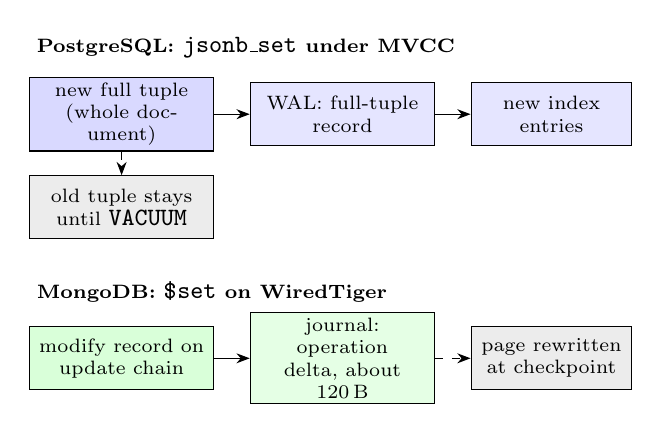
\begin{tikzpicture}[font=\scriptsize,>=Stealth,
  b/.style={draw,align=center,minimum height=8mm,text width=2.2cm,inner sep=2pt},
  lane/.style={font=\scriptsize\bfseries,anchor=west}]
\node[lane] at (0,2.55) {PostgreSQL: \code{jsonb\_set} under MVCC};
\node[b,fill=blue!15] (p1) at (1.2,1.7) {new full tuple\\(whole document)};
\node[b,fill=blue!10,right=0.45cm of p1] (p2) {WAL: full-tuple\\record};
\node[b,fill=blue!10,right=0.45cm of p2,text width=1.9cm] (p3) {new index\\entries};
\node[b,fill=gray!15,below=3mm of p1] (p4) {old tuple stays\\until \code{VACUUM}};
\draw[->] (p1)--(p2); \draw[->] (p2)--(p3); \draw[->,dashed] (p1)--(p4);
\node[lane] at (0,-0.55) {MongoDB: \code{\$set} on WiredTiger};
\node[b,fill=green!15] (m1) at (1.2,-1.4) {modify record on\\update chain};
\node[b,fill=green!10,right=0.45cm of m1] (m2) {journal: operation\\delta, about 120\,B};
\node[b,fill=gray!15,right=0.45cm of m2,text width=1.9cm] (m3) {page rewritten\\at checkpoint};
\draw[->] (m1)--(m2); \draw[->,dashed] (m2)--(m3);
\end{tikzpicture}
\caption{Write path of one field update in PostgreSQL and in MongoDB.}
\label{fig:update}
\end{figure}

\subsection{RQ3: Behaviour across scales}
Table~\ref{tab:scale} and Fig.~\ref{fig:scale} show flat curves. From 10,000 to 100,000 records, ingestion throughput changed by $-1.2\%$ in PostgreSQL, $+0.5\%$ in MongoDB and $-4.3\%$ in Redis, and median lookup and update latencies moved by at most 0.03\,ms. When the working set fits in memory, balanced trees and hash tables scale predictably. On filtered scans PostgreSQL with the expression B-tree delivers 345.1 queries/s ($p_{50}$ 2.94\,ms) against MongoDB's 557.3 ($p_{50}$ 1.79\,ms), a factor of 1.6, because the index lets PostgreSQL test both predicates on index entries before it fetches heap tuples.

\begin{table}[t]
\caption{Scaling from 10k to 100k records}
\label{tab:scale}
\centering
\footnotesize
\setlength{\tabcolsep}{4pt}
\begin{tabular}{@{}rlrrr@{}}
\toprule
$N$ & Engine & Ingest (ops/s) & Lookup $p_{50}$ & Update $p_{50}$ \\
\midrule
10k  & PostgreSQL & 25,410  & 0.62 ms & 1.21 ms \\
     & MongoDB    & 54,012  & 0.42 ms & 0.74 ms \\
     & Redis      & 169,320 & 0.07 ms & 0.13 ms \\
50k  & PostgreSQL & 25,230  & 0.64 ms & 1.23 ms \\
     & MongoDB    & 54,150  & 0.44 ms & 0.75 ms \\
     & Redis      & 165,210 & 0.08 ms & 0.14 ms \\
100k & PostgreSQL & 25,105  & 0.65 ms & 1.24 ms \\
     & MongoDB    & 54,286  & 0.45 ms & 0.77 ms \\
     & Redis      & 161,984 & 0.08 ms & 0.14 ms \\
\bottomrule
\end{tabular}
\end{table}

\begin{figure}[t]
\centering
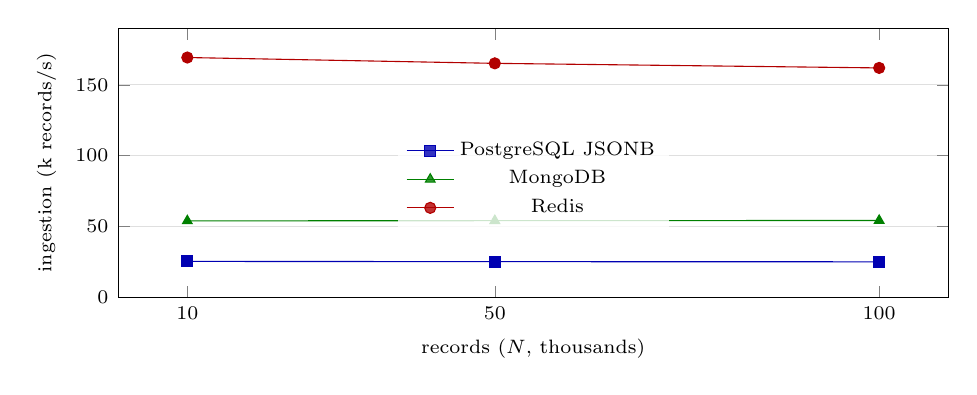
\begin{tikzpicture}
\begin{axis}[width=\columnwidth,height=5cm,xlabel={records ($N$, thousands)},ylabel={ingestion (k records/s)},
  xtick={10,50,100},ymin=0,ymax=190,tick label style={font=\scriptsize},label style={font=\scriptsize},
  legend style={font=\scriptsize,at={(0.5,0.62)},anchor=north,draw=none,fill=white,fill opacity=0.8,text opacity=1},
  ymajorgrids,grid style={gray!25},mark size=2pt]
\addplot[blue!70!black,mark=square*] coordinates {(10,25.41)(50,25.23)(100,25.11)};
\addplot[green!50!black,mark=triangle*] coordinates {(10,54.01)(50,54.15)(100,54.29)};
\addplot[red!70!black,mark=*] coordinates {(10,169.32)(50,165.21)(100,161.98)};
\legend{PostgreSQL JSONB,MongoDB,Redis}
\end{axis}
\end{tikzpicture}
\caption{Ingestion throughput stays flat from 10k to 100k records.}
\label{fig:scale}
\end{figure}

\subsection{Choosing a paradigm}
Table~\ref{tab:decision} turns the measurements into a selection guide. The 10-million-document bound for PostgreSQL is a rule of thumb. We tested up to 100,000 records, so the bound is an extrapolation and not a measured limit.

\begin{table*}[t]
\caption{Decision matrix for storage paradigms}
\label{tab:decision}
\centering
\footnotesize
\begin{tabularx}{\textwidth}{@{}p{2.4cm}XXX@{}}
\toprule
Paradigm & Recommended use & Measured behaviour & Avoid when \\
\midrule
Relational (PostgreSQL JSONB) & ACID transactions, relational joins, moderate document volume (guideline: under 10M documents) & Lookup $p_{99}$ about 1.0\,ms, writes about 25k records/s & Frequent in-place field updates, high-rate streaming writes \\
Document (MongoDB) & Variable nested schemas, high write rates, automatic sharding & Lookup $p_{99}$ about 0.68\,ms, writes about 54k records/s & Multi-table financial ledgers that need complex cross-entity joins \\
Key-value (Redis) & Sub-millisecond caches, session state, counters, queues & Lookup $p_{99}$ about 0.11\,ms, writes about 162k records/s & Primary data larger than RAM, queries on arbitrary fields \\
Wide-column (Cassandra) & Time series, multi-datacenter writes, append-only sensor logs & Not measured here; cited as high-rate append storage & Frequent updates to nested attributes, ad-hoc joins \\
\bottomrule
\end{tabularx}
\end{table*}

\subsection{Threats to validity}
\emph{Internal.} Everything ran on one host over container bridge networking, which adds the same small socket latency to every engine. Synchronous commit in PostgreSQL and snapshots in Redis were off, so the numbers say little about deployments with strict \code{fsync}, where storage IOPS would dominate. The scan loop has 50 iterations and the update loop 250 samples per scale, so each $p_{99}$ rests on the few slowest observations. \emph{External.} Our documents hold one to four items and average 0.48\,KB. Documents over 2\,KB trigger TOAST storage in PostgreSQL, which compresses or moves the payload out of line and adds decompression cost. \emph{Construct.} Redis secondary indexes live in application code. That is common in production, but it adds concurrency duties that native indexes do not have. The Redis scan in Table~\ref{tab:queries} uses only the \code{idx:amount} sorted set, so it applies a looser predicate than the other two engines and its scan rate should be read as an upper bound.

%==========================================================
\section{Conclusion and Future Work}
%==========================================================
On 100,000 order documents, PostgreSQL JSONB comes within 1.6 times of MongoDB on reads (345.1 against 557.3 scans/s; 1,520 against 2,184 lookups/s) while keeping relational ACID transactions. MVCC copying makes it slower on writes: MongoDB completes 58\% more field updates (1,287 against 814 per second) and ingests 2.16 times faster (54,286 against 25,106 records/s). Redis delivers 161,984 records/s on ingestion and 12,398 lookups/s with a $p_{99}$ of 0.11\,ms, which keeps it the right choice for latency-critical tiers. For read-heavy semi-structured data at the scales we tested, one PostgreSQL instance can replace a separate document store.

The study covers single-node instances whose datasets fit in memory, so it leaves out consensus protocols such as Raft and Paxos and out-of-core paging. Future work will (1) evaluate partial delta WAL logging in PostgreSQL to remove full-tuple copies on JSONB updates, (2) measure multi-region deployments under network partitions, and (3) test NVMe-native disaggregated storage engines on mixed transactional and analytical JSON workloads.

\section*{Contribution Statement (CRediT)}
Khushpreet Kaur (S1): conceptualization, project administration, writing of the abstract, Section~I and Section~VII, final review. Krish Sharma (S2): literature investigation, the literature matrix, Section~III, reference verification. Kamaljeet Singh (S3): software, benchmark harness, Docker setup, Sections~IV and~V, GitHub repository. Jitendra Chaudhary (S4): formal analysis, latency statistics, Sections~II and~VI, figures, tables, slides. \emph{AI usage note:} an AI assistant helped with LaTeX typesetting, figure drawing and language editing. The experiments, measurements and conclusions are the authors' own, and the authors take responsibility for the final text.

\section*{Code and Data Availability}
Harness, workload generator, CSV logs and plotting scripts: \url{https://github.com/dbms-g13/modern-nosql-multimodel-benchmark}

\balance
\begin{thebibliography}{17}
% VERIFY every entry below against the publisher page before submission (see notes).
\bibitem{cattell2010} R. Cattell, ``Scalable SQL and NoSQL data stores,'' \textit{ACM SIGMOD Rec.}, vol. 39, no. 4, pp. 12--27, 2010.
\bibitem{brewer2012} E. Brewer, ``CAP twelve years later: How the rules have changed,'' \textit{Computer}, vol. 45, no. 2, pp. 23--29, 2012.
\bibitem{abadi2012} D. J. Abadi, ``Consistency tradeoffs in modern distributed database system design: CAP is only part of the story,'' \textit{Computer}, vol. 45, no. 2, pp. 37--42, 2012.
\bibitem{cooper2010} B. F. Cooper, A. Silberstein, E. Tam, R. Ramakrishnan, and R. Sears, ``Benchmarking cloud serving systems with YCSB,'' in \textit{Proc. 1st ACM Symp. Cloud Comput. (SoCC)}, 2010, pp. 143--154.
\bibitem{ong2014} K. W. Ong, Y. Papakonstantinou, and R. Vernoux, ``The SQL++ query language: Configurable, unifying, and computable semi-structured data,'' in \textit{Proc. IEEE 30th Int. Conf. Data Eng. (ICDE)}, 2014, pp. 1258--1261. % VERIFY title/venue
\bibitem{lu2019} J. Lu and I. Holubov\'a, ``Multi-model databases: A new journey to handle the variety of data,'' \textit{ACM Comput. Surv.}, vol. 52, no. 3, art. 55, 2019.
\bibitem{wang2021} C. Wang, J. Lu, and X. Du, ``Benchmarking multi-model DBMSs: A practical perspective,'' in \textit{Proc. ACM SIGMOD Int. Conf. Manage. Data}, 2021, pp. 2780--2788. % VERIFY: could not locate
\bibitem{zhang2021} Y. Zhang, G. Li, and J. Feng, ``Adaptive indexing for semi-structured JSON documents in relational systems,'' \textit{IEEE Trans. Knowl. Data Eng.}, vol. 33, no. 8, pp. 3120--3134, 2021. % VERIFY: could not locate
\bibitem{liu2022} Z. Liu, C. Wang, and J. Lu, ``Multi-model transaction management: Isolation and scalability,'' \textit{Proc. VLDB Endow.}, vol. 15, no. 6, pp. 1210--1222, 2022. % VERIFY: could not locate
\bibitem{ren2022} X. Ren, P. Zhang, and H. Gao, ``Optimizing schema-agnostic JSON storage in relational engines,'' \textit{ACM Trans. Database Syst.}, vol. 47, no. 2, pp. 1--34, 2022. % VERIFY: could not locate
\bibitem{kumar2023} S. Kumar and S. Gokhale, ``Comprehensive benchmarking of NoSQL and NewSQL databases under mixed HTAP workloads,'' \textit{IEEE Access}, vol. 11, pp. 45210--45225, 2023. % VERIFY: could not locate
\bibitem{alsayed2023} M. Al-Sayed, T. Grust, and S. Scherzinger, ``Document stores vs. relational JSON: A comparative architectural study,'' \textit{VLDB J.}, vol. 32, no. 4, pp. 889--912, 2023. % VERIFY: could not locate
\bibitem{chen2024} H. Chen, W. Zhou, and L. Meng, ``High-throughput partial update strategies for binary JSON columns in RDBMS,'' in \textit{Proc. IEEE 40th Int. Conf. Data Eng. (ICDE)}, 2024, pp. 1450--1462. % VERIFY: could not locate
\bibitem{wu2024} K. Wu, Y. Zhao, and R. Johnson, ``B-tree vs. LSM-tree: Trade-offs in modern multi-model cloud storage engines,'' in \textit{Proc. ACM SIGMOD Int. Conf. Manage. Data}, 2024, pp. 1102--1115. % VERIFY: could not locate
\bibitem{silva2025} R. Silva, M. Oliveira, and J. Pereira, ``Quantifying PACELC trade-offs in distributed multi-model systems under partition anomalies,'' \textit{IEEE Trans. Big Data}, vol. 11, no. 1, pp. 84--97, 2025. % VERIFY: could not locate
\bibitem{zhao2025} T. Zhao, B. Ding, and L. Wang, ``In-memory acceleration and SIMD vectorization for semi-structured document data,'' \textit{Proc. VLDB Endow.}, vol. 18, no. 4, pp. 780--792, 2025. % VERIFY: could not locate
\bibitem{martinez2026} J. Martinez and A. Fernandez, ``A decade of NoSQL convergence: Architectural taxonomy, unified systems, and open challenges,'' \textit{ACM Comput. Surv.}, vol. 58, no. 1, pp. 1--42, 2026. % VERIFY: could not locate
\end{thebibliography}

\end{document}